\chapter{Second Design Iteration} \label{chapter:design-second-iteration}
The previous usability study revealed several usability issues that prevented users from achieving their goals. This chapter outlines how the most severe issues have been addressed and presents the revised interface design. The sections below are structured based on the different feature areas of the interface. Figure \ref{fig:main-views-diagram} might help to visualize the relations between them: The main editing view as well as the diff comparison are very central, whereas the remaining features are more or less equally important. Please note that the diff is not an independent view of itself but is embedded in several other views, such as the history, the saving page and the merge request details.

\begin{figure}[h!]
 \centering
 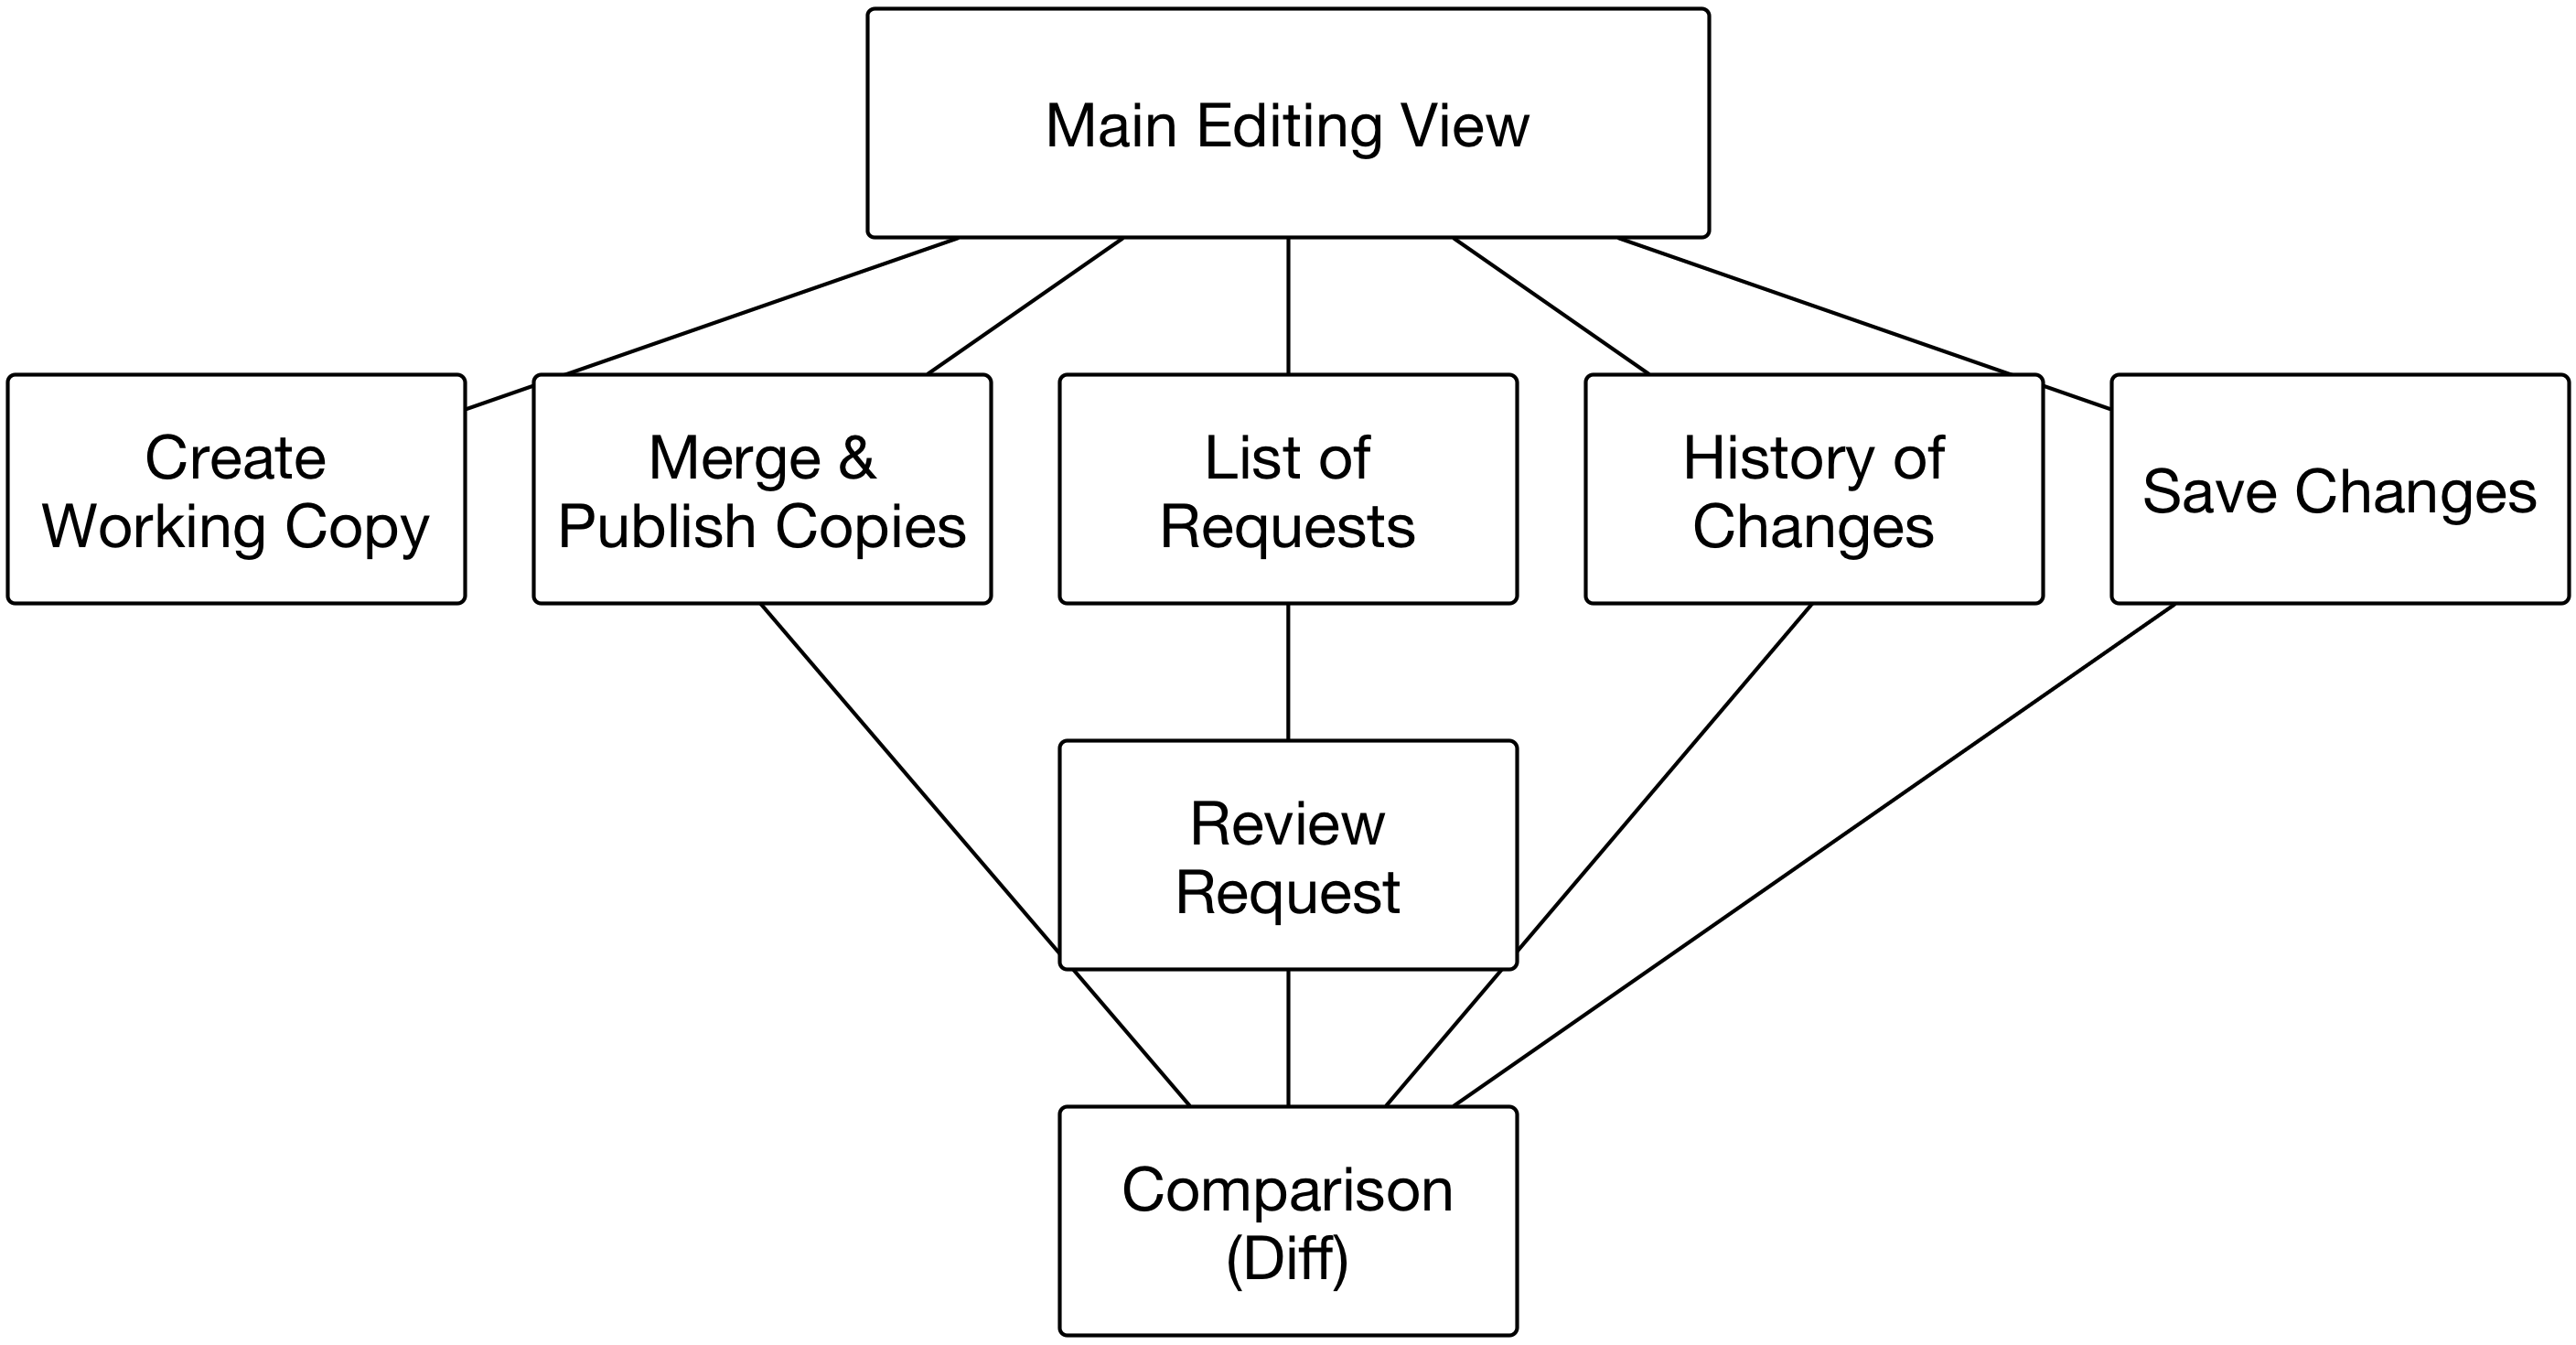
\includegraphics[width=11cm]{second-iteration/main-views-diagram}
 \caption{Main parts of the application}
 \label{fig:main-views-diagram}
\end{figure}

%In addition, Section \ref{sec:navigation-revised-terminology} highlights how the results of the focus group influenced the new terminology used within the interface.

%Additionally a lot of smaller changes were done as well, such as improving error messages, rephrasing explanations or reordering certain elements within views.

%As compared to the first prototype, the design was no longer just black and white, but utilized the Babbel corporate identity, so that it was closer to how a finished tool would look like. Additionally, the interface went from a semi-interactive prototype, based on graphical layouts, to a fully interactive web application. The prototype was based on AngularJS \cite{_angularjs_????}, a framework initially intended to facilitate rapid prototyping, which has evolved into a full-fledged frontend framework for developing single page web applications. These applications feel much more like Desktop-Applications than Websites, because new content is loaded asynchronously and therefore there is no visible interruption when navigating the app. The prototype was not fully functional, but covered the main version control features like its predecessor.

% \section{Usability Issues}
% Table \ref{sec:navigation-revised-terminology} shows the most problematic usability issues of each feature area discovered during the previous study. The table is sorted by the issue number and the following sections refer to these issues numbers to underline what problems have been solved by redesigning the different interface parts.

% \begin{table}[h!]
% \centering
% \begin{tabular}{|l|p{6cm}|l|l|l|}
% \hline
% \rowcolor[HTML]{EFEFEF}
% \textbf{\#} & \textbf{Usability issue} & \textbf{Feature area} & \textbf{Impact} \\ \hline
% 1 & Create new branch button was not found & Branches (Working Copies) & 40 \\ \hline
% 2 & Warning about editing content inside the master branch was ignored & Branches (Working Copies) & 40 \\ \hline
% 6 & Concept of a pull request is not clear (term might be confusing) & Pull Request & 40 \\ \hline
% 11 & New translations listed in the diff view are confusing, because the left column is empty (some users expected to see the learning language text) & Diff & 80 \\ \hline
% 12 & Not clear how to get from the diff view to the editing view & Diff & 40 \\ \hline
% 14 & Save button was not found (expected at bottom of screen) & Saving Process & 80 \\ \hline
% 19 & Visual representation/hierarchy of items/exercises not entirely clear & Main editing view & 18 \\ \hline
% 23 & Main navigation not completely obvious, clicking through (trial \& error) & Navigation & 20 \\ \hline
% \end{tabular}
% \caption{Usability issues with the highest impact scores from each feature area}
% \label{table:issues-most-impact-first-study}
% \end{table}

\section{Navigation and Terminology} \label{sec:navigation-revised-terminology}
During the first usability study as well as the subsequent focus group, the version control terminology has been identified as a major usability issue (Issues \#4, \#6 and \#23). Users especially struggled with grasping the concepts behind branches and pull requests. Based on the results and the input from the focus group, new names were conceived for some of the main features. Most notably, branches are now called working copies, or just copies, and pull requests are referred to as merge or publish requests. The term copy was chosen, because it is part of everyday language and much less abstract than the term branch. "Pull" was swapped for "merge" or "publish", because it describes the action of combining two different states of the content much better.

Additionally, the names of most features now signify an action (unsaved changes is now save changes, pull requests is now review requests, create pull request is now merge or publish). The intention behind this was to signal the result of an action to the user upfront and thus allow him or her to anticipate the result of an interaction.

Besides improving the used terminology, the design of the navigation bar was also slightly tweaked. Most importantly, all items now have labels and icons that visualize the feature, which could help users to orient themselves in a better way (Issues \#1 and \#25). Because this takes more space now, the repository (language package) selection has been moved to the upper right corner (Figure \ref{fig:nav-bar-old-new}).

\begin{figure}[h!]
 \centering
 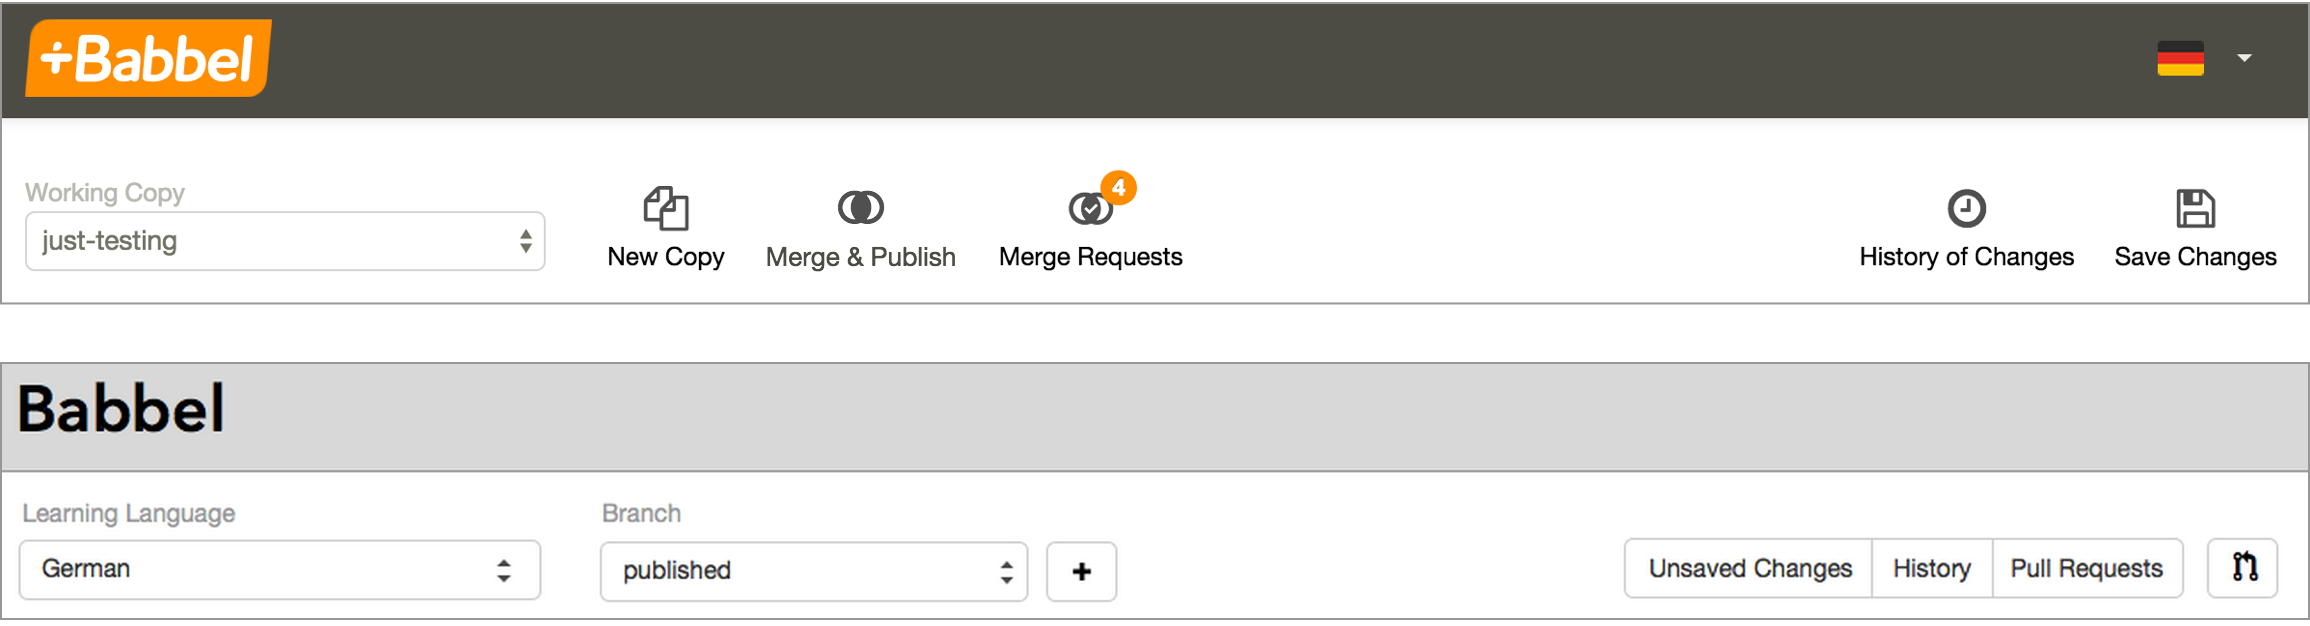
\includegraphics[width=\textwidth]{second-iteration/changes/nav-bar-old-new}
 \caption{New and old navigation bar}
 \label{fig:nav-bar-old-new}
\end{figure}

\section{Branches/Working Copies}
During the previous usability study the branch concept presented some serious problems to users. First of all, most participants were confused when being informed that editing the main branch is not possible (Issue \#2) and just ignored the message. Afterwards, many took some time till finding the functionality of creating a new branch (Issue \#1).

The warning message in the previous prototype (Figure \ref{fig:live-data-warning}) did not offer any solutions to the users. This lead to a situation where many users were lost after the message appeared. In order to mitigate this problem the new warning message now offers solutions right away. Users can choose to create a new working copy or dismiss the warning and edit the live content anyway.

Additionally the main branch was renamed from \emph{master} to \emph{published} to make it even clearer which kind of content is inside, thus fixing Issue \#3 and \#4.



%In most version control systems it is regarded as a best practice to make changes only on feature branches and thus keeping the main branch (master) always in a functional state. The same workflow is desired for content authoring since the public content should always be in an error-free state so that Babbel end-users always get the best possible experience. Not editing the live content directly thus reduces the risk of introducing new errors and allows collaborators to review changes before they are merged. For this reason, a warning message informs users when they are editing the main branch. This warning lead to some confusion during the first usability study. Users noticed they had

%In order to make the version control capabilities of the new content authoring tool as easy to use as possible the system offers a lot of explanations and assists users in making the right decisions. For example there is a warning when users are editing the live content/main branch (Figure \ref{fig:live-data-warning}).



\begin{figure}[h!]
 \centering
 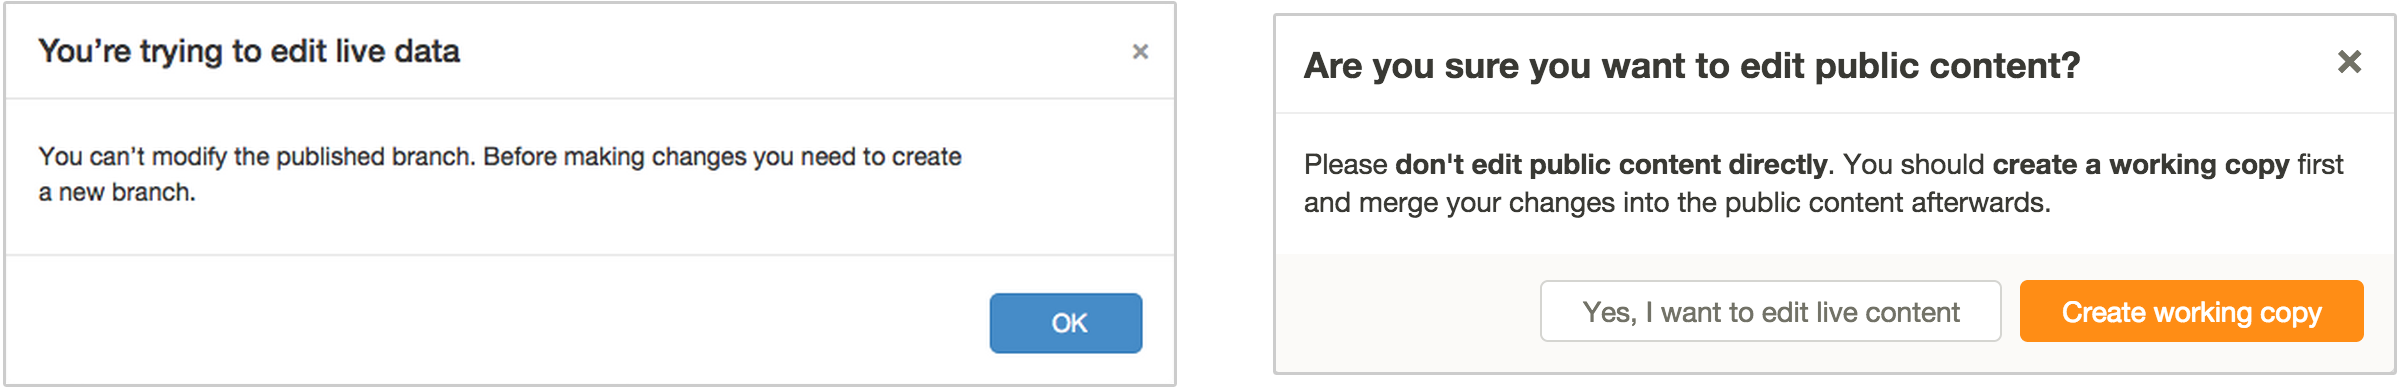
\includegraphics[width=\textwidth]{second-iteration/changes/live-data-warning}
 \caption{Live data warning old vs. new}
 \label{fig:live-data-warning}
\end{figure}

% \section{Issue \#6: Updated Terminology} \label{sec:changed-terminology}
% The focus group gathered after the first usability study made clear that the technical version control terminology used for the first prototype is only poorly understood. Therefore, new terms were conceived for the features least understood. In general, these were branches and pull requests.

\section{Improved Diff View}
The diff view posed some problems to users when looking at added translations (Issue \#11). Because the previous state was no translation at all the view showed a red empty box. Some users mistook this for a missing translation or an indication of an error, because of the red color (Issue \#13). The new design used a gray box instead to show that there was nothing before (Figure \ref{fig:improved-diff-view}).

Issue \#12, which prevented users from navigating from the diff view to the editing view, was addressed by underlining the breadcrumb, so that it became clearer that one can interact with it. Furthermore, instead of the button saying "show item" it was now labeled "edit lesson", which is hopefully clearer as well.

\begin{figure}[h!]
 \centering
 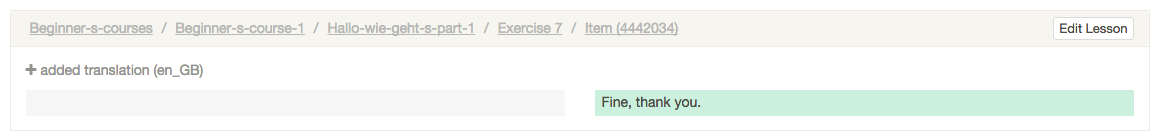
\includegraphics[width=\textwidth]{second-iteration/changes/improved-diff}
 \caption{Improved diff view}
 \label{fig:improved-diff-view}
\end{figure}

\section{Saving Process}
As Figure \ref{fig:saving-shortcut} shows the editor view now offers a shortcut for saving changes. In the design of the first iteration users were forced to use the save changes view (Figure \ref{fig:save-changes}), which also shows the differences between the old and the new state of the content. This is of course useful if a lot of changes have been done, especially across several lessons. But, the last study has shown, that users do not necessarily work that way (Issue \#18) and that it is often more convenient to save small changes right away. Therefore a simple save button at the bottom of the content table was introduced.

Furthermore, Issue \#16, which was related to the naming of the "back to editor" button and the fact that users confused its meaning with a "real" content editor, was solved by using a simple \emph{x} instead, which is often used for closing views or popups.

\begin{figure}[h!]
 \centering
 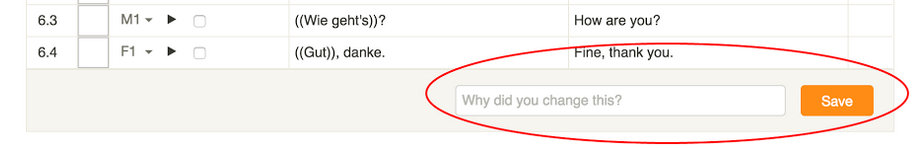
\includegraphics[width=\textwidth]{second-iteration/changes/saving-shortcut}
 \caption{Saving shortcut}
 \label{fig:saving-shortcut}
\end{figure}

\begin{figure}[hp!]
 \centering
 \fbox{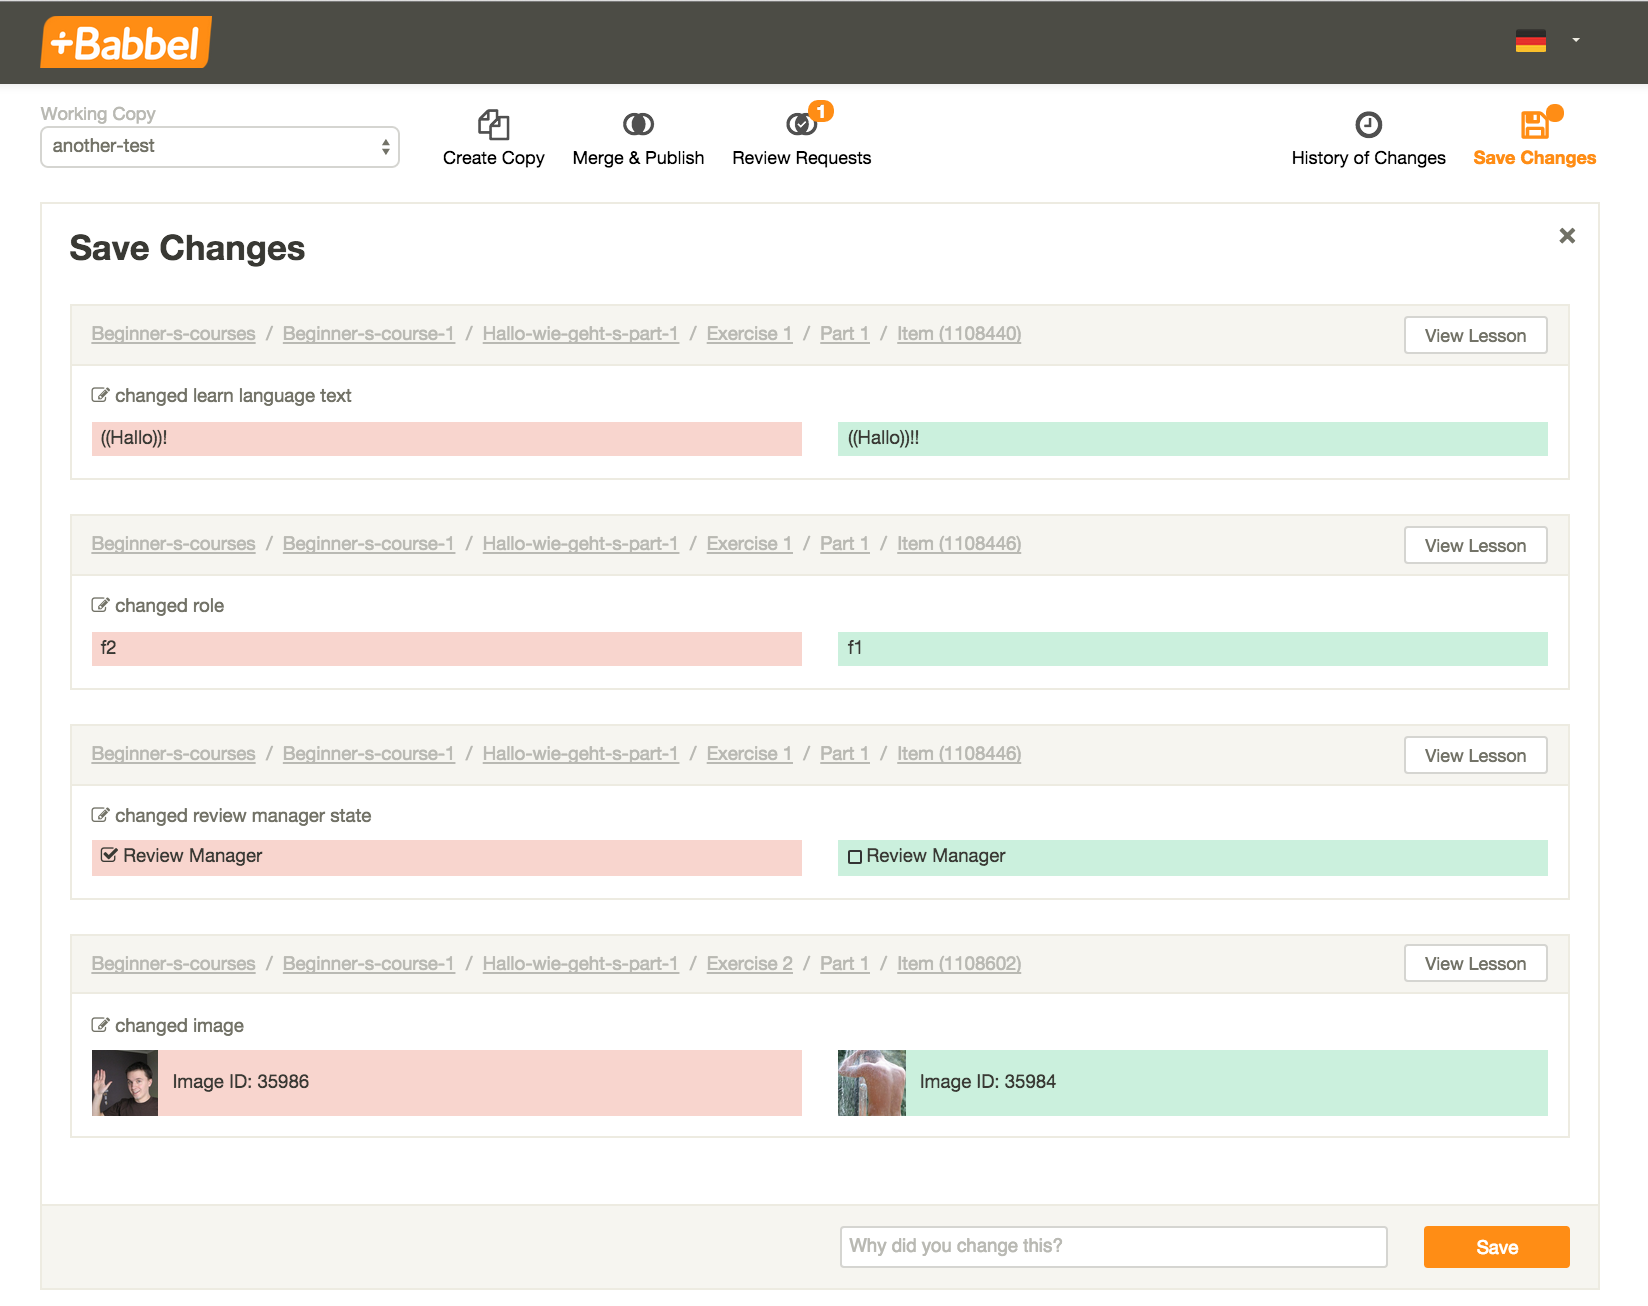
\includegraphics[width=\textwidth]{second-iteration/save-changes}}
 \caption{Save changes}
 \label{fig:save-changes}
\end{figure}

\section{New Content Representation}
For the new interface a different content representation was designed (Figure \ref{fig:main-editing-view}). The old one, which was using so called accordions, hid a lot of information in the beginning. According to the Yahoo Developer Network, the main reason for using accordions is "to compress a large amount of options into a limited space" \cite{_accordion_2009}. This design pattern has the advantage to provide users with a quick overview, but the downside is that some information can only be exposed through a user interaction. Bret Victor explained this phenomenon as "harmful interaction" and provides the insight that good software design is often just good graphic design \cite{victor_magic_2006}. The accordions were one of the reasons why Scenario 3 presented such a hurdle for most users during the last study (Issues \#19 and \#20). Therefore, the new design uses a table layout which presents most of the important information at a glance. The intention is to provide a better overview without necessary interaction and thus enable users to find errors or problems in the overall lesson structure more quickly. Furthermore, this spreadsheet-like design should be very familiar to most users, since spreadsheets were used a lot as an auxiliary tool before, as described in Section \ref{sec:task1}.

% \section{Visualisations}
% Even though the visualisations were appreciated by the participants in the first user study, they were changed in the new interface. This is due to the fact that branches are now called copies and the old visualisations might have been confusing in conjunction with this slightly changed concept. Therefore the visualisations were swapped for simpler icons that indicate what is happening. Creating a new working copy is now visualised by two file symbols lying on top of each other (Figure \ref{fig:working-copy-creation}). The merging view now shows an icon similar to a Venn diagram, which indicates that only the differences between the first and the second copy will be merged into the second one.

% \begin{figure}[h!]
%  \centering
%  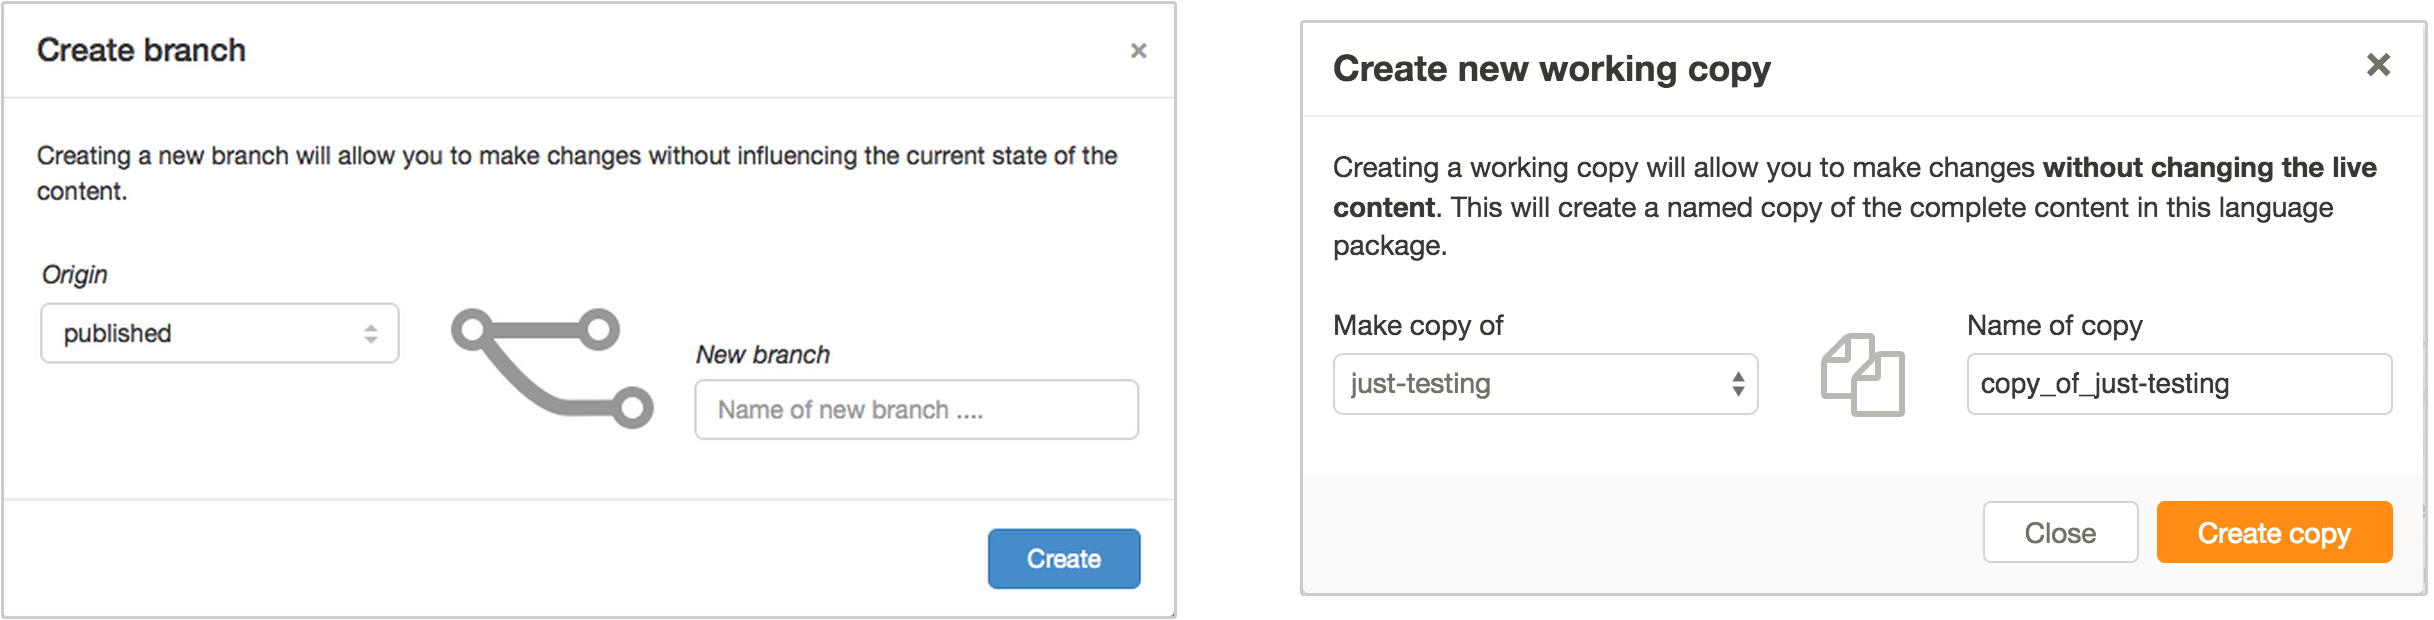
\includegraphics[width=\textwidth]{second-iteration/changes/working-copy-creation}
%  \caption{Creating branches/copies old vs. new}
%  \label{fig:working-copy-creation}
% \end{figure}

% \begin{figure}[h!]
%  \centering
%  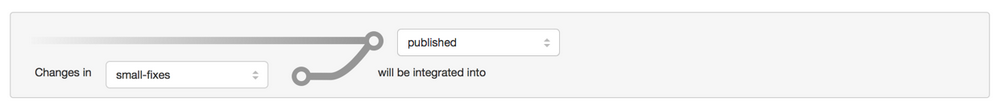
\includegraphics[width=\textwidth]{second-iteration/changes/merge-vis-old}
%  \caption{Merging branches old design}
%  \label{fig:merge-vis-old}
% \end{figure}

% \begin{figure}[h!]
%  \centering
%  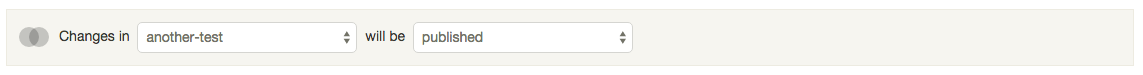
\includegraphics[width=\textwidth]{second-iteration/changes/merge-vis-new}
%  \caption{Merging copies new design}
%  \label{fig:merge-vis-new}
% \end{figure}


\begin{figure}[hp!]
 \centering
 \fbox{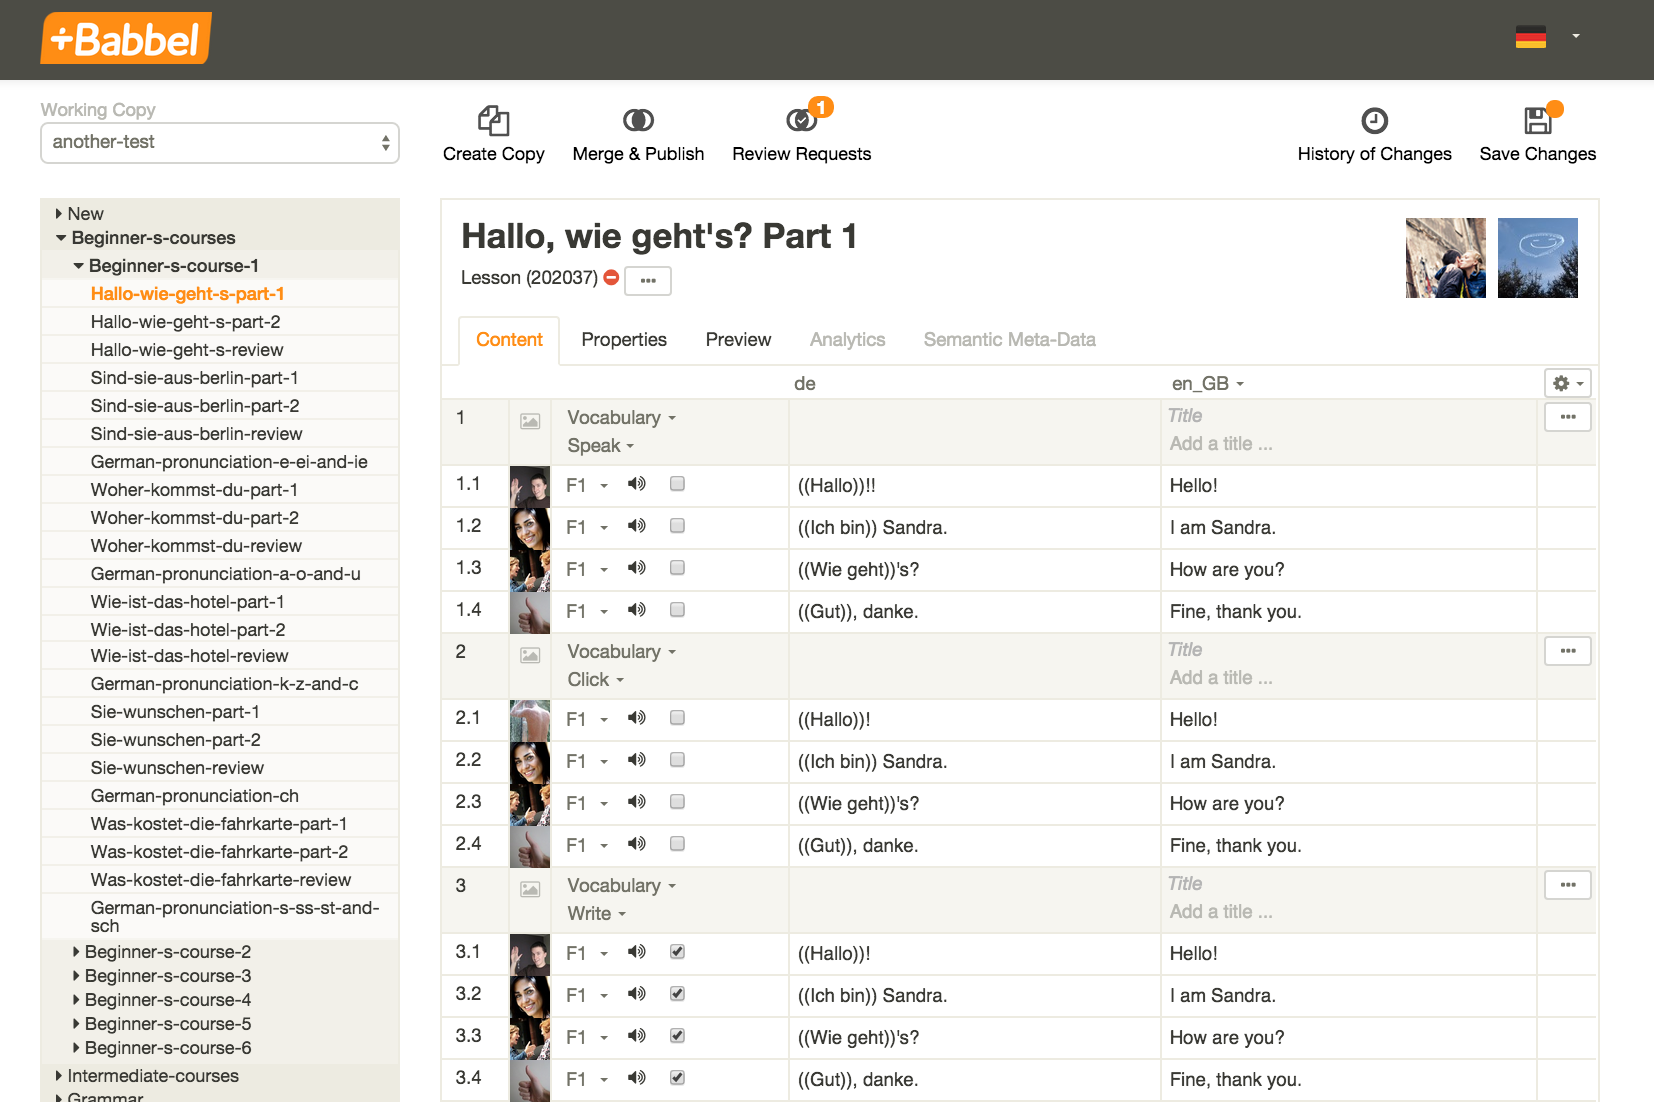
\includegraphics[width=\textwidth]{second-iteration/content-editing}}
 \caption{Main editing view}
 \label{fig:main-editing-view}
\end{figure}

\begin{figure}[hp!]
 \centering
 \fbox{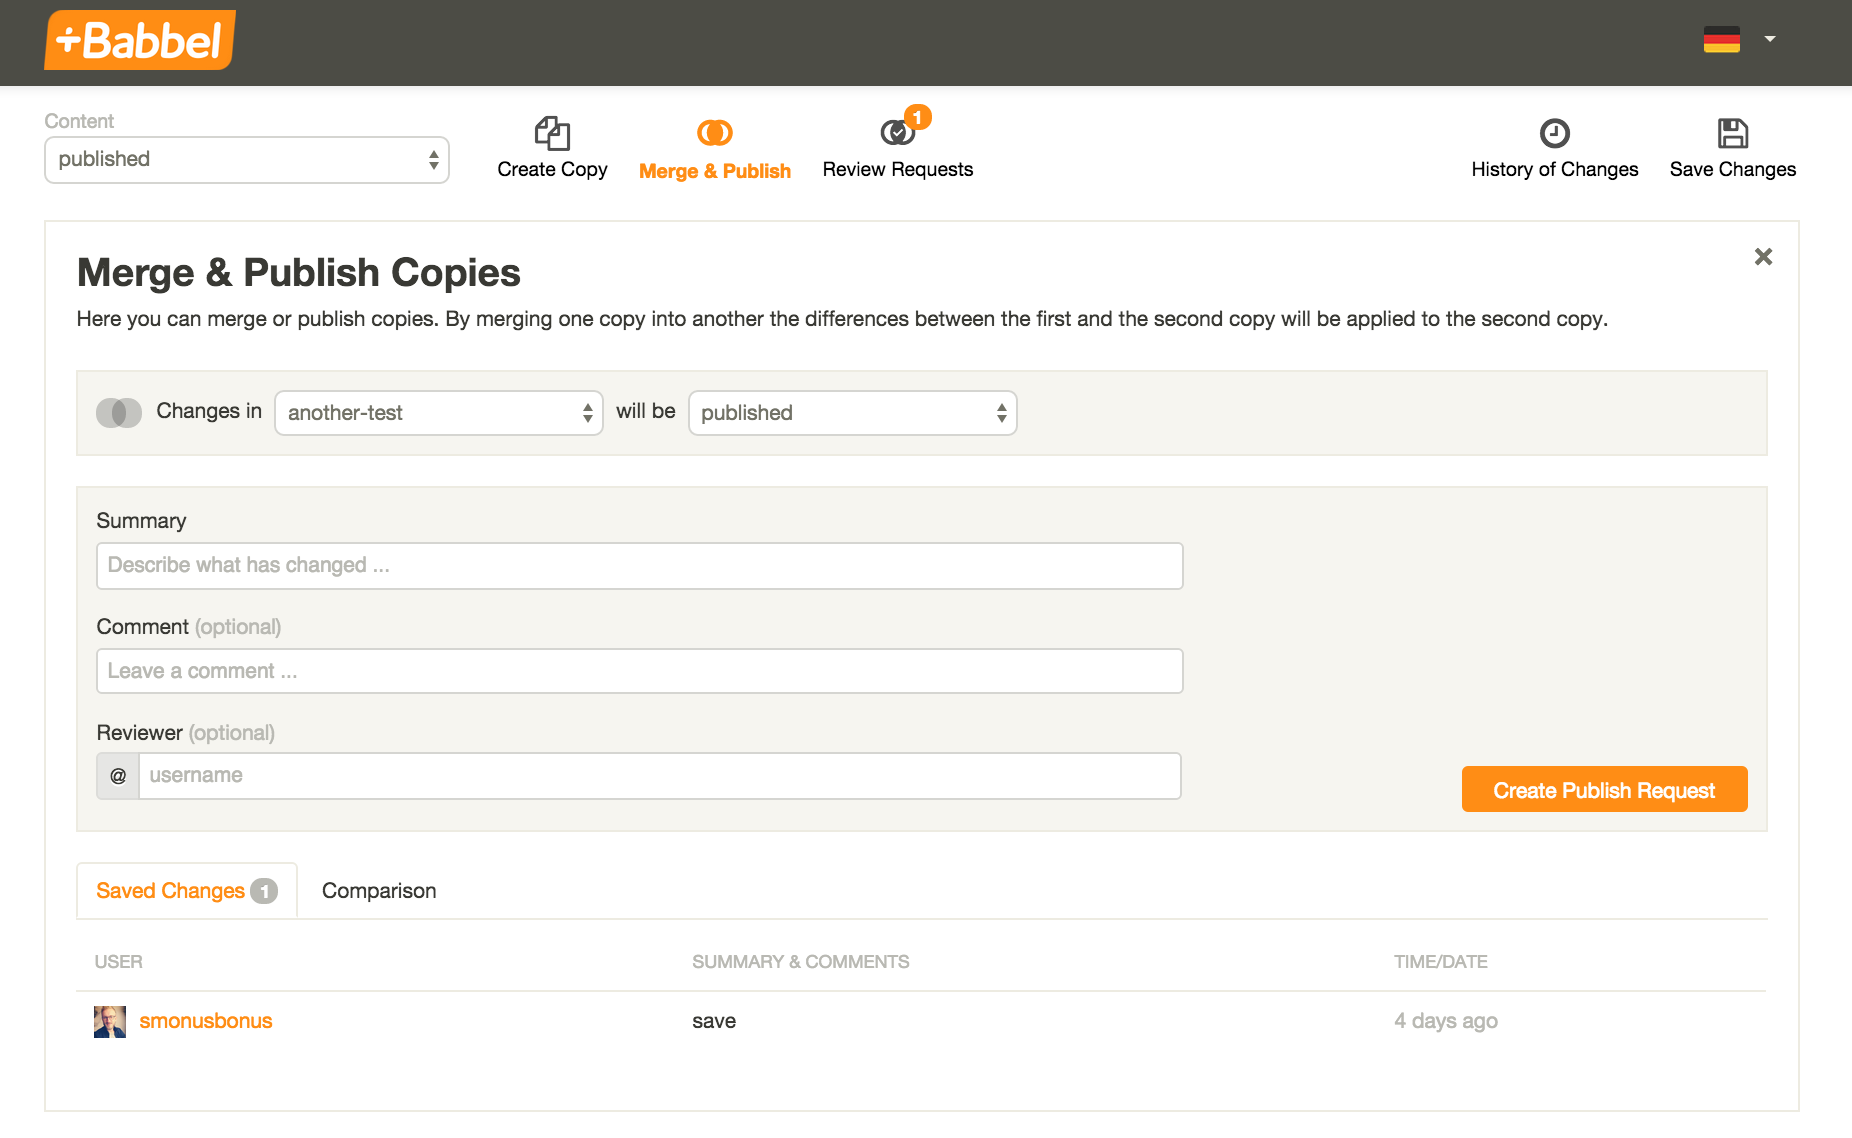
\includegraphics[width=\textwidth]{second-iteration/merge-copies}}
 \caption{Merge or publish copies}
\end{figure}

% \begin{figure}[hp!]
%  \centering
%  \fbox{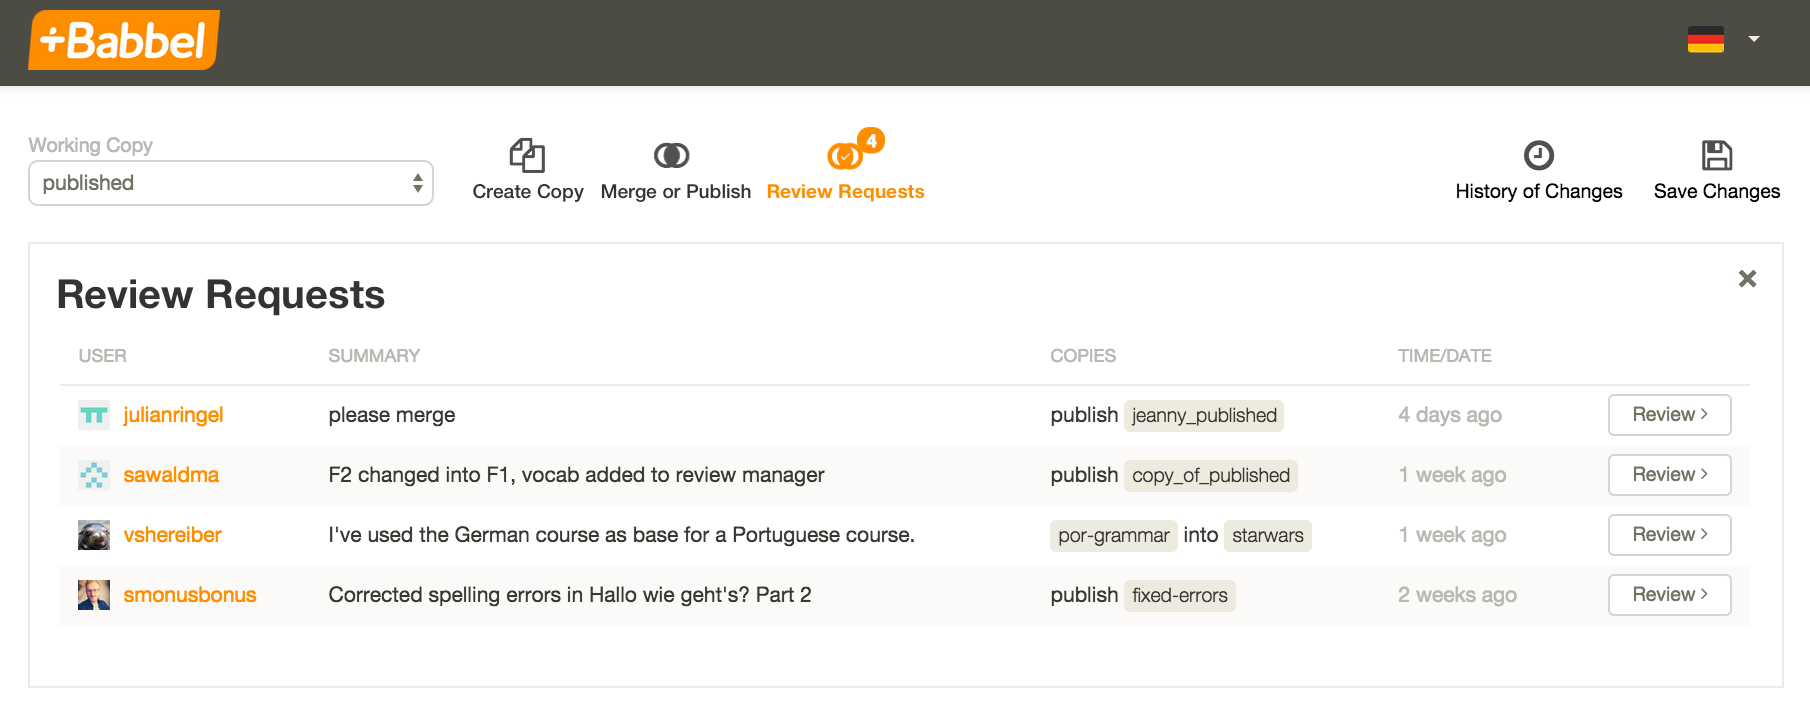
\includegraphics[width=\textwidth]{second-iteration/list-of-requests}}
%  \caption{List of requests}
% \end{figure}

\begin{figure}[hp!]
 \centering
 \fbox{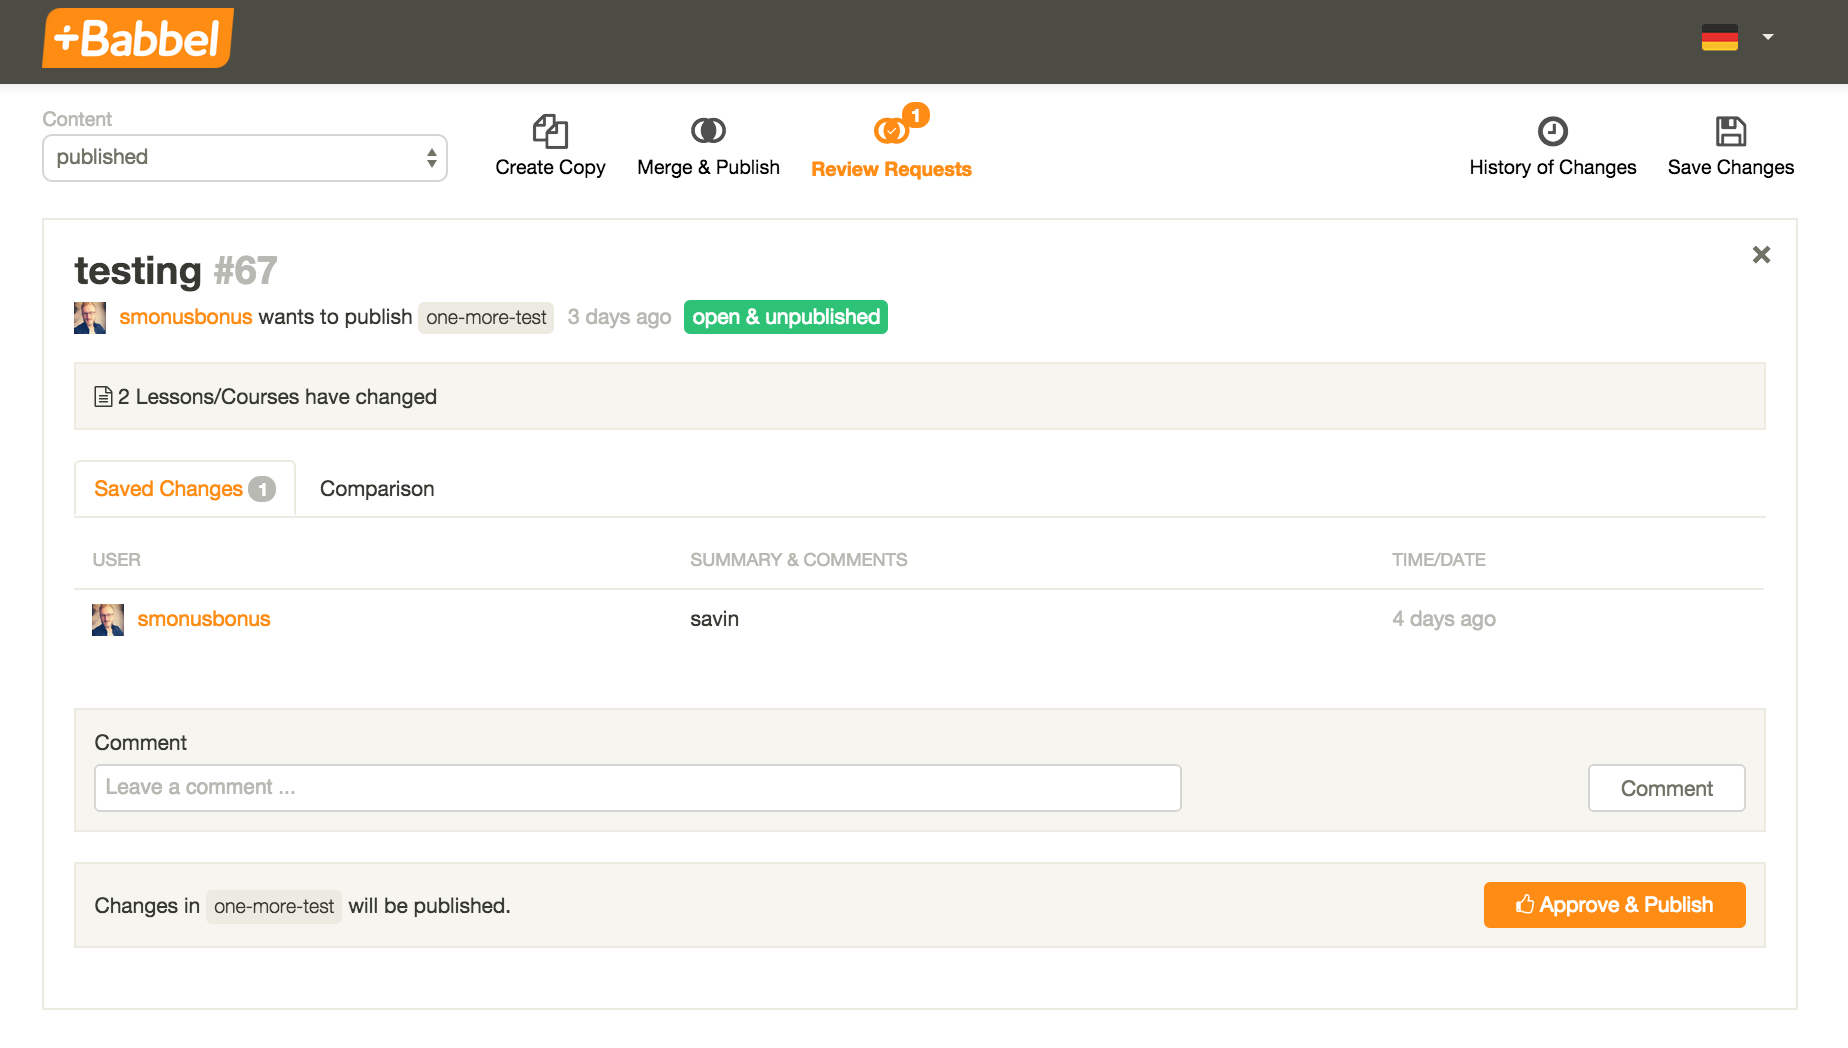
\includegraphics[width=\textwidth]{second-iteration/request-detail}}
 \caption{Review request}
\end{figure}
